\documentclass[1p]{elsarticle_modified}
%\bibliographystyle{elsarticle-num}

%\usepackage[colorlinks]{hyperref}
%\usepackage{abbrmath_seonhwa} %\Abb, \Ascr, \Acal ,\Abf, \Afrak
\usepackage{amsfonts}
\usepackage{amssymb}
\usepackage{amsmath}
\usepackage{amsthm}
\usepackage{scalefnt}
\usepackage{amsbsy}
\usepackage{kotex}
\usepackage{caption}
\usepackage{subfig}
\usepackage{color}
\usepackage{graphicx}
\usepackage{xcolor} %% white, black, red, green, blue, cyan, magenta, yellow
\usepackage{float}
\usepackage{setspace}
\usepackage{hyperref}

\usepackage{tikz}
\usetikzlibrary{arrows}

\usepackage{multirow}
\usepackage{array} % fixed length table
\usepackage{hhline}

%%%%%%%%%%%%%%%%%%%%%
\makeatletter
\renewcommand*\env@matrix[1][\arraystretch]{%
	\edef\arraystretch{#1}%
	\hskip -\arraycolsep
	\let\@ifnextchar\new@ifnextchar
	\array{*\c@MaxMatrixCols c}}
\makeatother %https://tex.stackexchange.com/questions/14071/how-can-i-increase-the-line-spacing-in-a-matrix
%%%%%%%%%%%%%%%

\usepackage[normalem]{ulem}

\newcommand{\msout}[1]{\ifmmode\text{\sout{\ensuremath{#1}}}\else\sout{#1}\fi}
%SOURCE: \msout is \stkout macro in https://tex.stackexchange.com/questions/20609/strikeout-in-math-mode

\newcommand{\cancel}[1]{
	\ifmmode
	{\color{red}\msout{#1}}
	\else
	{\color{red}\sout{#1}}
	\fi
}

\newcommand{\add}[1]{
	{\color{blue}\uwave{#1}}
}

\newcommand{\replace}[2]{
	\ifmmode
	{\color{red}\msout{#1}}{\color{blue}\uwave{#2}}
	\else
	{\color{red}\sout{#1}}{\color{blue}\uwave{#2}}
	\fi
}

\newcommand{\Sol}{\mathcal{S}} %segment
\newcommand{\D}{D} %diagram
\newcommand{\A}{\mathcal{A}} %arc


%%%%%%%%%%%%%%%%%%%%%%%%%%%%%5 test

\def\sl{\operatorname{\textup{SL}}(2,\Cbb)}
\def\psl{\operatorname{\textup{PSL}}(2,\Cbb)}
\def\quan{\mkern 1mu \triangleright \mkern 1mu}

\theoremstyle{definition}
\newtheorem{thm}{Theorem}[section]
\newtheorem{prop}[thm]{Proposition}
\newtheorem{lem}[thm]{Lemma}
\newtheorem{ques}[thm]{Question}
\newtheorem{cor}[thm]{Corollary}
\newtheorem{defn}[thm]{Definition}
\newtheorem{exam}[thm]{Example}
\newtheorem{rmk}[thm]{Remark}
\newtheorem{alg}[thm]{Algorithm}

\newcommand{\I}{\sqrt{-1}}
\begin{document}

%\begin{frontmatter}
%
%\title{Boundary parabolic representations of knots up to 8 crossings}
%
%%% Group authors per affiliation:
%\author{Yunhi Cho} 
%\address{Department of Mathematics, University of Seoul, Seoul, Korea}
%\ead{yhcho@uos.ac.kr}
%
%
%\author{Seonhwa Kim} %\fnref{s_kim}}
%\address{Center for Geometry and Physics, Institute for Basic Science, Pohang, 37673, Korea}
%\ead{ryeona17@ibs.re.kr}
%
%\author{Hyuk Kim}
%\address{Department of Mathematical Sciences, Seoul National University, Seoul 08826, Korea}
%\ead{hyukkim@snu.ac.kr}
%
%\author{Seokbeom Yoon}
%\address{Department of Mathematical Sciences, Seoul National University, Seoul, 08826,  Korea}
%\ead{sbyoon15@snu.ac.kr}
%
%\begin{abstract}
%We find all boundary parabolic representation of knots up to 8 crossings.
%
%\end{abstract}
%\begin{keyword}
%    \MSC[2010] 57M25 
%\end{keyword}
%
%\end{frontmatter}

%\linenumbers
%\tableofcontents
%
\newcommand\colored[1]{\textcolor{white}{\rule[-0.35ex]{0.8em}{1.4ex}}\kern-0.8em\color{red} #1}%
%\newcommand\colored[1]{\textcolor{white}{ #1}\kern-2.17ex	\textcolor{white}{ #1}\kern-1.81ex	\textcolor{white}{ #1}\kern-2.15ex\color{red}#1	}

{\Large $\underline{11a_{102}~(K11a_{102})}$}

\setlength{\tabcolsep}{10pt}
\renewcommand{\arraystretch}{1.6}
\vspace{1cm}\begin{tabular}{m{100pt}>{\centering\arraybackslash}m{274pt}}
\multirow{5}{120pt}{
	\centering
	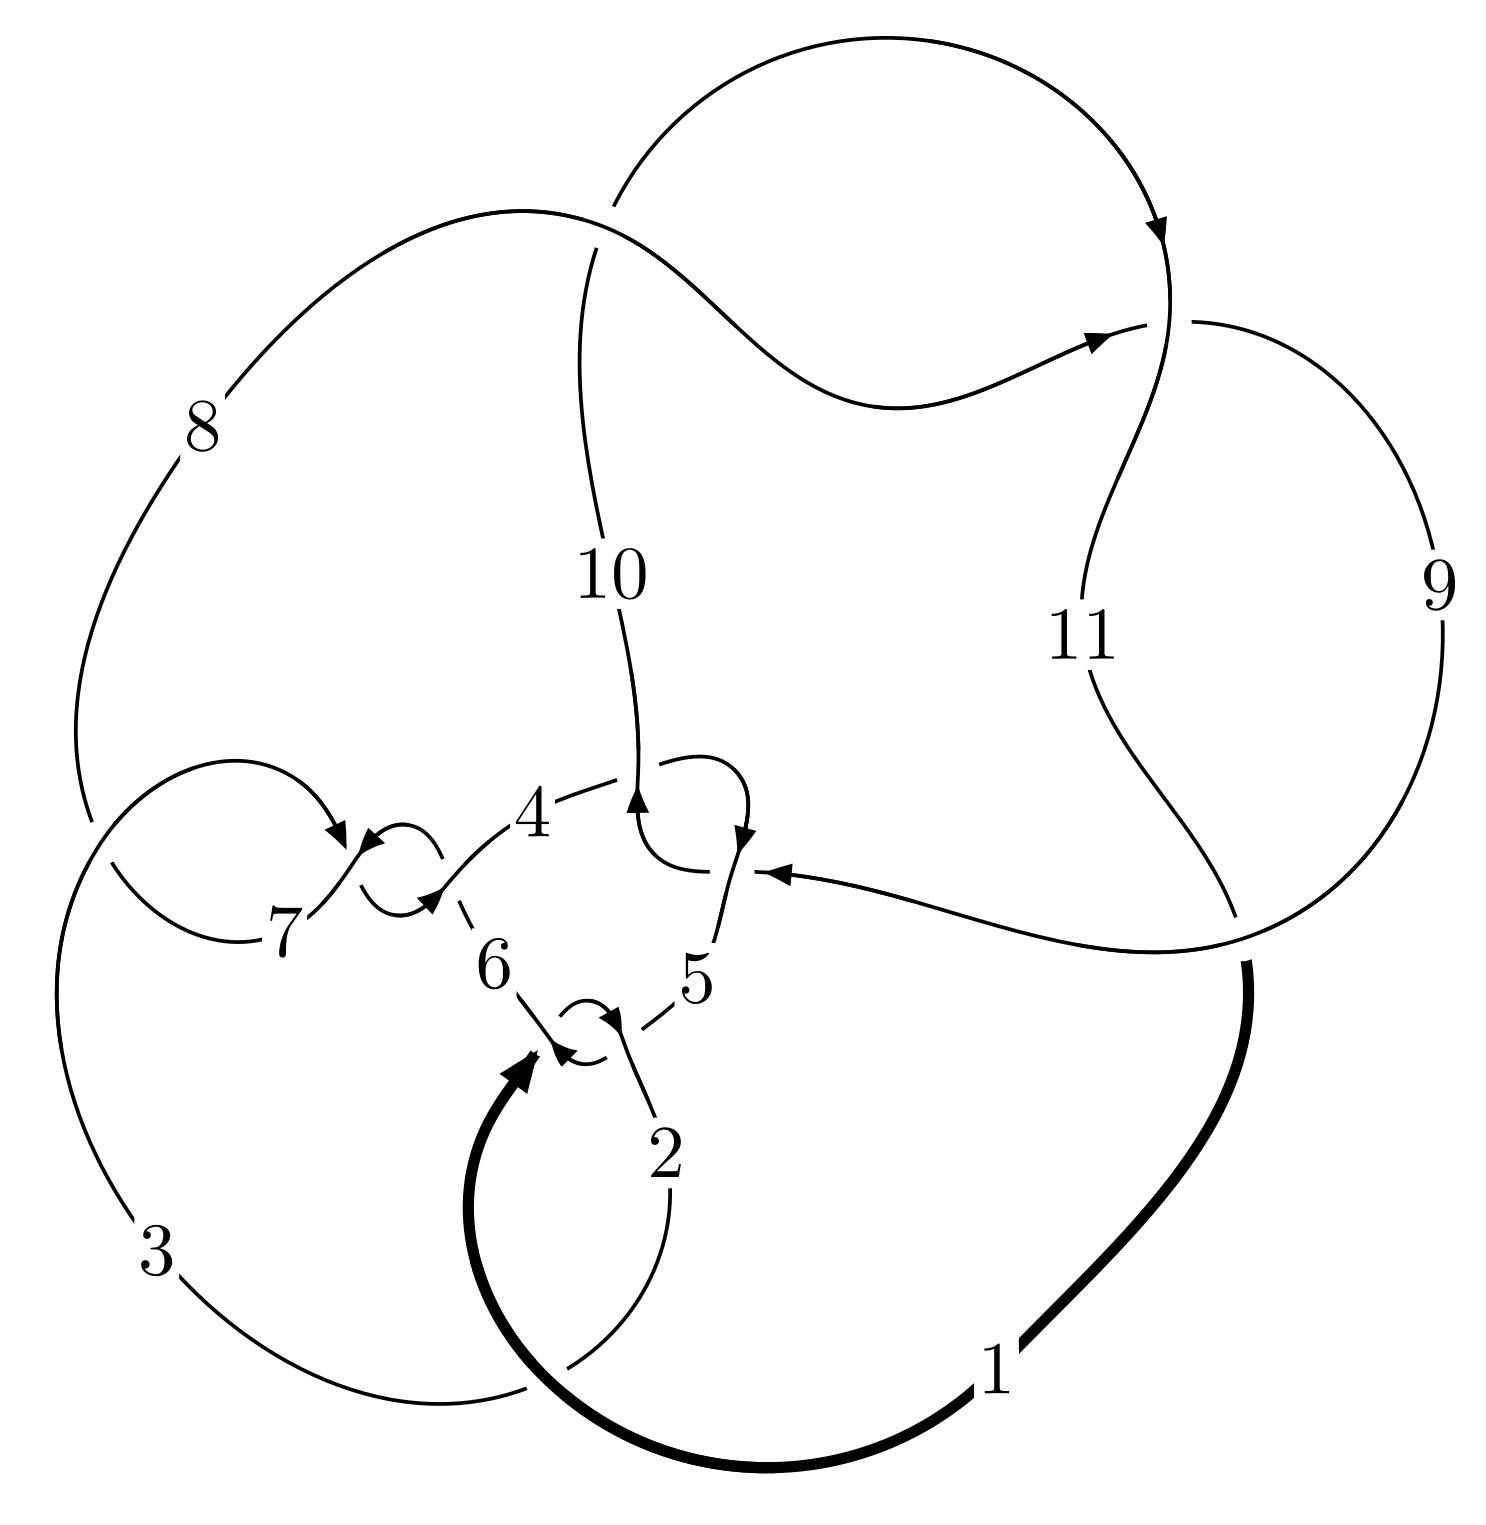
\includegraphics[width=112pt]{../../../GIT/diagram.site/Diagrams/png/351_11a_102.png}\\
\ \ \ A knot diagram\footnotemark}&
\allowdisplaybreaks
\textbf{Linearized knot diagam} \\
\cline{2-2}
 &
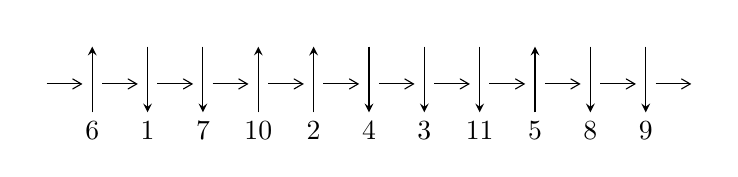
\begin{tikzpicture}[x=20pt, y=17pt]
	% nodes
	\node (C0) at (0, 0) {};
	\node (C1) at (1, 0) {};
	\node (C1U) at (1, +1) {};
	\node (C1D) at (1, -1) {6};

	\node (C2) at (2, 0) {};
	\node (C2U) at (2, +1) {};
	\node (C2D) at (2, -1) {1};

	\node (C3) at (3, 0) {};
	\node (C3U) at (3, +1) {};
	\node (C3D) at (3, -1) {7};

	\node (C4) at (4, 0) {};
	\node (C4U) at (4, +1) {};
	\node (C4D) at (4, -1) {10};

	\node (C5) at (5, 0) {};
	\node (C5U) at (5, +1) {};
	\node (C5D) at (5, -1) {2};

	\node (C6) at (6, 0) {};
	\node (C6U) at (6, +1) {};
	\node (C6D) at (6, -1) {4};

	\node (C7) at (7, 0) {};
	\node (C7U) at (7, +1) {};
	\node (C7D) at (7, -1) {3};

	\node (C8) at (8, 0) {};
	\node (C8U) at (8, +1) {};
	\node (C8D) at (8, -1) {11};

	\node (C9) at (9, 0) {};
	\node (C9U) at (9, +1) {};
	\node (C9D) at (9, -1) {5};

	\node (C10) at (10, 0) {};
	\node (C10U) at (10, +1) {};
	\node (C10D) at (10, -1) {8};

	\node (C11) at (11, 0) {};
	\node (C11U) at (11, +1) {};
	\node (C11D) at (11, -1) {9};
	\node (C12) at (12, 0) {};

	% arrows
	\draw[->,>={angle 60}]
	(C0) edge (C1) (C1) edge (C2) (C2) edge (C3) (C3) edge (C4) (C4) edge (C5) (C5) edge (C6) (C6) edge (C7) (C7) edge (C8) (C8) edge (C9) (C9) edge (C10) (C10) edge (C11) (C11) edge (C12) ;	\draw[->,>=stealth]
	(C1D) edge (C1U) (C2U) edge (C2D) (C3U) edge (C3D) (C4D) edge (C4U) (C5D) edge (C5U) (C6U) edge (C6D) (C7U) edge (C7D) (C8U) edge (C8D) (C9D) edge (C9U) (C10U) edge (C10D) (C11U) edge (C11D) ;
	\end{tikzpicture} \\
\hhline{~~} \\& 
\textbf{Solving Sequence} \\ \cline{2-2} 
 &
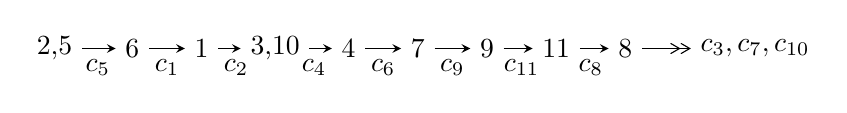
\begin{tikzpicture}[x=25pt, y=7pt]
	% node
	\node (A0) at (-1/8, 0) {2,5};
	\node (A1) at (1, 0) {6};
	\node (A2) at (2, 0) {1};
	\node (A3) at (49/16, 0) {3,10};
	\node (A4) at (33/8, 0) {4};
	\node (A5) at (41/8, 0) {7};
	\node (A6) at (49/8, 0) {9};
	\node (A7) at (57/8, 0) {11};
	\node (A8) at (65/8, 0) {8};
	\node (C1) at (1/2, -1) {$c_{5}$};
	\node (C2) at (3/2, -1) {$c_{1}$};
	\node (C3) at (5/2, -1) {$c_{2}$};
	\node (C4) at (29/8, -1) {$c_{4}$};
	\node (C5) at (37/8, -1) {$c_{6}$};
	\node (C6) at (45/8, -1) {$c_{9}$};
	\node (C7) at (53/8, -1) {$c_{11}$};
	\node (C8) at (61/8, -1) {$c_{8}$};
	\node (A9) at (10, 0) {$c_{3},c_{7},c_{10}$};

	% edge
	\draw[->,>=stealth]	
	(A0) edge (A1) (A1) edge (A2) (A2) edge (A3) (A3) edge (A4) (A4) edge (A5) (A5) edge (A6) (A6) edge (A7) (A7) edge (A8) ;
	\draw[->>,>={angle 60}]	
	(A8) edge (A9);
\end{tikzpicture} \\ 

\end{tabular} \\

\footnotetext{
The image of knot diagram is generated by the software ``\textbf{Draw programme}" developed by Andrew Bartholomew(\url{http://www.layer8.co.uk/maths/draw/index.htm\#Running-draw}), where we modified some parts for our purpose(\url{https://github.com/CATsTAILs/LinksPainter}).
}\phantom \\ \newline 
\centering \textbf{Ideals for irreducible components\footnotemark of $X_{\text{par}}$} 
 
\begin{align*}
I^u_{1}&=\langle 
2.87536\times10^{21} u^{41}-3.96737\times10^{21} u^{40}+\cdots+5.90778\times10^{21} b-6.72165\times10^{21},\\
\phantom{I^u_{1}}&\phantom{= \langle  }2.13130\times10^{22} u^{41}-4.18187\times10^{22} u^{40}+\cdots+7.08933\times10^{22} a-3.54422\times10^{23},\;u^{42}-2 u^{41}+\cdots-36 u+9\rangle \\
I^u_{2}&=\langle 
- u^{12}-4 u^{10}-3 u^9-6 u^8-9 u^7-7 u^6-9 u^5-7 u^4-3 u^3-3 u^2+b+1,\\
\phantom{I^u_{2}}&\phantom{= \langle  }- u^{13}- u^{12}-4 u^{11}-6 u^{10}-8 u^9-12 u^8-11 u^7-11 u^6-9 u^5-3 u^4- u^3+u^2+a+3 u+1,\\
\phantom{I^u_{2}}&\phantom{= \langle  }u^{15}+5 u^{13}+3 u^{12}+10 u^{11}+12 u^{10}+14 u^9+18 u^8+17 u^7+13 u^6+13 u^5+5 u^4+3 u^3+u^2- u-1\rangle \\
I^u_{3}&=\langle 
b,\;u^3+2 u^2+2 a+3 u+1,\;u^4+u^3+u^2+1\rangle \\
I^u_{4}&=\langle 
a u+5 b-2 a-3 u+1,\;a^2- a+5 u+4,\;u^2+1\rangle \\
\\
\end{align*}
\raggedright * 4 irreducible components of $\dim_{\mathbb{C}}=0$, with total 65 representations.\\
\footnotetext{All coefficients of polynomials are rational numbers. But the coefficients are sometimes approximated in decimal forms when there is not enough margin.}
\newpage
\renewcommand{\arraystretch}{1}
\centering \section*{I. $I^u_{1}= \langle 2.88\times10^{21} u^{41}-3.97\times10^{21} u^{40}+\cdots+5.91\times10^{21} b-6.72\times10^{21},\;2.13\times10^{22} u^{41}-4.18\times10^{22} u^{40}+\cdots+7.09\times10^{22} a-3.54\times10^{23},\;u^{42}-2 u^{41}+\cdots-36 u+9 \rangle$}
\flushleft \textbf{(i) Arc colorings}\\
\begin{tabular}{m{7pt} m{180pt} m{7pt} m{180pt} }
\flushright $a_{2}=$&$\begin{pmatrix}0\\u\end{pmatrix}$ \\
\flushright $a_{5}=$&$\begin{pmatrix}1\\0\end{pmatrix}$ \\
\flushright $a_{6}=$&$\begin{pmatrix}1\\- u^2\end{pmatrix}$ \\
\flushright $a_{1}=$&$\begin{pmatrix}- u\\u^3+u\end{pmatrix}$ \\
\flushright $a_{3}=$&$\begin{pmatrix}- u^3\\u^5+u^3+u\end{pmatrix}$ \\
\flushright $a_{10}=$&$\begin{pmatrix}-0.300635 u^{41}+0.589882 u^{40}+\cdots-15.7376 u+4.99938\\-0.486707 u^{41}+0.671550 u^{40}+\cdots-9.85137 u+1.13776\end{pmatrix}$ \\
\flushright $a_{4}=$&$\begin{pmatrix}0.279236 u^{41}-0.941462 u^{40}+\cdots+18.2040 u-4.05148\\0.463095 u^{41}-1.13764 u^{40}+\cdots+27.2892 u-7.18073\end{pmatrix}$ \\
\flushright $a_{7}=$&$\begin{pmatrix}0.797859 u^{41}-1.13262 u^{40}+\cdots+15.2674 u-0.433684\\0.308200 u^{41}-0.215226 u^{40}+\cdots-6.59502 u+3.37739\end{pmatrix}$ \\
\flushright $a_{9}=$&$\begin{pmatrix}0.186072 u^{41}-0.0816676 u^{40}+\cdots-5.88625 u+3.86161\\-0.486707 u^{41}+0.671550 u^{40}+\cdots-9.85137 u+1.13776\end{pmatrix}$ \\
\flushright $a_{11}=$&$\begin{pmatrix}-0.377575 u^{41}+0.483319 u^{40}+\cdots+4.32261 u-2.55226\\-0.157428 u^{41}+0.0210348 u^{40}+\cdots+8.77277 u-2.82010\end{pmatrix}$ \\
\flushright $a_{8}=$&$\begin{pmatrix}0.626320 u^{41}-0.755435 u^{40}+\cdots+11.7778 u+0.221051\\0.157428 u^{41}-0.0210348 u^{40}+\cdots-8.77277 u+2.82010\end{pmatrix}$\\ \flushright $a_{8}=$&$\begin{pmatrix}0.626320 u^{41}-0.755435 u^{40}+\cdots+11.7778 u+0.221051\\0.157428 u^{41}-0.0210348 u^{40}+\cdots-8.77277 u+2.82010\end{pmatrix}$\\&\end{tabular}
\flushleft \textbf{(ii) Obstruction class $= -1$}\\~\\
\flushleft \textbf{(iii) Cusp Shapes $= \frac{3375308932150515076741}{15754069295721805208896} u^{41}-\frac{7093505981346082336715}{15754069295721805208896} u^{40}+\cdots-\frac{990909890095625692917289}{15754069295721805208896} u+\frac{306048621353866106187553}{15754069295721805208896}$}\\~\\
\newpage\renewcommand{\arraystretch}{1}
\flushleft \textbf{(iv) u-Polynomials at the component}\newline \\
\begin{tabular}{m{50pt}|m{274pt}}
Crossings & \hspace{64pt}u-Polynomials at each crossing \\
\hline $$\begin{aligned}c_{1},c_{5}\end{aligned}$$&$\begin{aligned}
&u^{42}-2 u^{41}+\cdots-36 u+9
\end{aligned}$\\
\hline $$\begin{aligned}c_{2}\end{aligned}$$&$\begin{aligned}
&u^{42}+18 u^{41}+\cdots+936 u+81
\end{aligned}$\\
\hline $$\begin{aligned}c_{3},c_{6},c_{7}\end{aligned}$$&$\begin{aligned}
&u^{42}-2 u^{41}+\cdots-48 u+9
\end{aligned}$\\
\hline $$\begin{aligned}c_{4},c_{9}\end{aligned}$$&$\begin{aligned}
&u^{42}-2 u^{41}+\cdots-48 u+64
\end{aligned}$\\
\hline $$\begin{aligned}c_{8},c_{10},c_{11}\end{aligned}$$&$\begin{aligned}
&u^{42}-4 u^{41}+\cdots+3 u+4
\end{aligned}$\\
\hline
\end{tabular}\\~\\
\newpage\renewcommand{\arraystretch}{1}
\flushleft \textbf{(v) Riley Polynomials at the component}\newline \\
\begin{tabular}{m{50pt}|m{274pt}}
Crossings & \hspace{64pt}Riley Polynomials at each crossing \\
\hline $$\begin{aligned}c_{1},c_{5}\end{aligned}$$&$\begin{aligned}
&y^{42}+18 y^{41}+\cdots+936 y+81
\end{aligned}$\\
\hline $$\begin{aligned}c_{2}\end{aligned}$$&$\begin{aligned}
&y^{42}+18 y^{41}+\cdots+43092 y+6561
\end{aligned}$\\
\hline $$\begin{aligned}c_{3},c_{6},c_{7}\end{aligned}$$&$\begin{aligned}
&y^{42}+42 y^{41}+\cdots+648 y+81
\end{aligned}$\\
\hline $$\begin{aligned}c_{4},c_{9}\end{aligned}$$&$\begin{aligned}
&y^{42}+24 y^{41}+\cdots+37632 y+4096
\end{aligned}$\\
\hline $$\begin{aligned}c_{8},c_{10},c_{11}\end{aligned}$$&$\begin{aligned}
&y^{42}-40 y^{41}+\cdots+431 y+16
\end{aligned}$\\
\hline
\end{tabular}\\~\\
\newpage\flushleft \textbf{(vi) Complex Volumes and Cusp Shapes}
$$\begin{array}{c|c|c}  
\text{Solutions to }I^u_{1}& \I (\text{vol} + \sqrt{-1}CS) & \text{Cusp shape}\\
 \hline 
\begin{aligned}
u &= \phantom{-}0.321244 + 0.924907 I \\
a &= \phantom{-}0.68951 - 2.35177 I \\
b &= \phantom{-}0.16746 - 1.77078 I\end{aligned}
 & -8.34619 + 1.31277 I & -3.80780 - 5.75825 I \\ \hline\begin{aligned}
u &= \phantom{-}0.321244 - 0.924907 I \\
a &= \phantom{-}0.68951 + 2.35177 I \\
b &= \phantom{-}0.16746 + 1.77078 I\end{aligned}
 & -8.34619 - 1.31277 I & -3.80780 + 5.75825 I \\ \hline\begin{aligned}
u &= -0.781793 + 0.668749 I \\
a &= -0.179012 - 0.710623 I \\
b &= \phantom{-}0.864043 - 0.487802 I\end{aligned}
 & \phantom{-}6.85342 - 1.08907 I & \phantom{-}3.57208 + 1.87970 I \\ \hline\begin{aligned}
u &= -0.781793 - 0.668749 I \\
a &= -0.179012 + 0.710623 I \\
b &= \phantom{-}0.864043 + 0.487802 I\end{aligned}
 & \phantom{-}6.85342 + 1.08907 I & \phantom{-}3.57208 - 1.87970 I \\ \hline\begin{aligned}
u &= \phantom{-}0.786749 + 0.566093 I \\
a &= -0.122149 - 0.366661 I \\
b &= -0.176094 + 1.096880 I\end{aligned}
 & -4.33907 + 0.92313 I & -6.58218 - 1.96577 I \\ \hline\begin{aligned}
u &= \phantom{-}0.786749 - 0.566093 I \\
a &= -0.122149 + 0.366661 I \\
b &= -0.176094 - 1.096880 I\end{aligned}
 & -4.33907 - 0.92313 I & -6.58218 + 1.96577 I \\ \hline\begin{aligned}
u &= \phantom{-}1.010940 + 0.277119 I \\
a &= \phantom{-}0.118893 + 0.317524 I \\
b &= -0.708157 + 1.185080 I\end{aligned}
 & -0.13244 - 8.79986 I & -2.66885 + 5.03818 I \\ \hline\begin{aligned}
u &= \phantom{-}1.010940 - 0.277119 I \\
a &= \phantom{-}0.118893 - 0.317524 I \\
b &= -0.708157 - 1.185080 I\end{aligned}
 & -0.13244 + 8.79986 I & -2.66885 - 5.03818 I \\ \hline\begin{aligned}
u &= \phantom{-}0.443155 + 0.836892 I \\
a &= \phantom{-}0.077559 + 0.409124 I \\
b &= \phantom{-}0.533447 - 0.314098 I\end{aligned}
 & -0.14555 + 1.89662 I & -0.46549 - 4.15100 I \\ \hline\begin{aligned}
u &= \phantom{-}0.443155 - 0.836892 I \\
a &= \phantom{-}0.077559 - 0.409124 I \\
b &= \phantom{-}0.533447 + 0.314098 I\end{aligned}
 & -0.14555 - 1.89662 I & -0.46549 + 4.15100 I\\
 \hline 
 \end{array}$$\newpage$$\begin{array}{c|c|c}  
\text{Solutions to }I^u_{1}& \I (\text{vol} + \sqrt{-1}CS) & \text{Cusp shape}\\
 \hline 
\begin{aligned}
u &= \phantom{-}0.854547 + 0.372087 I \\
a &= \phantom{-}0.040427 - 0.627535 I \\
b &= \phantom{-}0.641022 - 1.066170 I\end{aligned}
 & \phantom{-}5.09584 - 4.47116 I & \phantom{-}1.35353 + 3.51083 I \\ \hline\begin{aligned}
u &= \phantom{-}0.854547 - 0.372087 I \\
a &= \phantom{-}0.040427 + 0.627535 I \\
b &= \phantom{-}0.641022 + 1.066170 I\end{aligned}
 & \phantom{-}5.09584 + 4.47116 I & \phantom{-}1.35353 - 3.51083 I \\ \hline\begin{aligned}
u &= -0.349226 + 1.057360 I \\
a &= \phantom{-}0.73971 + 2.07726 I \\
b &= -0.065056 + 1.043400 I\end{aligned}
 & -3.60913 - 1.10388 I & -10.34002 + 1.20607 I \\ \hline\begin{aligned}
u &= -0.349226 - 1.057360 I \\
a &= \phantom{-}0.73971 - 2.07726 I \\
b &= -0.065056 - 1.043400 I\end{aligned}
 & -3.60913 + 1.10388 I & -10.34002 - 1.20607 I \\ \hline\begin{aligned}
u &= \phantom{-}0.551141 + 1.033680 I \\
a &= -0.68540 + 2.16562 I \\
b &= \phantom{-}0.285987 + 1.305530 I\end{aligned}
 & \phantom{-}1.07465 + 4.16567 I & -3.63331 - 3.63134 I \\ \hline\begin{aligned}
u &= \phantom{-}0.551141 - 1.033680 I \\
a &= -0.68540 - 2.16562 I \\
b &= \phantom{-}0.285987 - 1.305530 I\end{aligned}
 & \phantom{-}1.07465 - 4.16567 I & -3.63331 + 3.63134 I \\ \hline\begin{aligned}
u &= \phantom{-}0.438210 + 1.089350 I \\
a &= -0.210411 - 0.547185 I \\
b &= -1.120410 + 0.266857 I\end{aligned}
 & -5.07603 + 3.61628 I & -8.76999 - 3.97464 I \\ \hline\begin{aligned}
u &= \phantom{-}0.438210 - 1.089350 I \\
a &= -0.210411 + 0.547185 I \\
b &= -1.120410 - 0.266857 I\end{aligned}
 & -5.07603 - 3.61628 I & -8.76999 + 3.97464 I \\ \hline\begin{aligned}
u &= \phantom{-}0.629402 + 0.513854 I \\
a &= -0.454894 + 1.264650 I \\
b &= -0.532736 + 1.051670 I\end{aligned}
 & \phantom{-}2.61565 + 0.48442 I & -1.18826 - 1.33056 I \\ \hline\begin{aligned}
u &= \phantom{-}0.629402 - 0.513854 I \\
a &= -0.454894 - 1.264650 I \\
b &= -0.532736 - 1.051670 I\end{aligned}
 & \phantom{-}2.61565 - 0.48442 I & -1.18826 + 1.33056 I\\
 \hline 
 \end{array}$$\newpage$$\begin{array}{c|c|c}  
\text{Solutions to }I^u_{1}& \I (\text{vol} + \sqrt{-1}CS) & \text{Cusp shape}\\
 \hline 
\begin{aligned}
u &= -0.705333 + 0.962448 I \\
a &= -0.390598 + 0.325640 I \\
b &= -0.865578 - 0.213500 I\end{aligned}
 & \phantom{-}5.99098 - 4.47238 I & \phantom{-}2.83567 + 4.51985 I \\ \hline\begin{aligned}
u &= -0.705333 - 0.962448 I \\
a &= -0.390598 - 0.325640 I \\
b &= -0.865578 + 0.213500 I\end{aligned}
 & \phantom{-}5.99098 + 4.47238 I & \phantom{-}2.83567 - 4.51985 I \\ \hline\begin{aligned}
u &= -0.715912 + 0.371485 I \\
a &= \phantom{-}0.682256 + 1.165700 I \\
b &= -1.056740 + 0.582481 I\end{aligned}
 & \phantom{-}1.90495 + 2.38439 I & -0.748912 - 0.739188 I \\ \hline\begin{aligned}
u &= -0.715912 - 0.371485 I \\
a &= \phantom{-}0.682256 - 1.165700 I \\
b &= -1.056740 - 0.582481 I\end{aligned}
 & \phantom{-}1.90495 - 2.38439 I & -0.748912 + 0.739188 I \\ \hline\begin{aligned}
u &= -0.515614 + 1.080020 I \\
a &= -1.12031 - 1.77848 I \\
b &= \phantom{-}0.439748 - 1.104040 I\end{aligned}
 & -2.45148 - 5.86761 I & -6.25811 + 7.21816 I \\ \hline\begin{aligned}
u &= -0.515614 - 1.080020 I \\
a &= -1.12031 + 1.77848 I \\
b &= \phantom{-}0.439748 + 1.104040 I\end{aligned}
 & -2.45148 + 5.86761 I & -6.25811 - 7.21816 I \\ \hline\begin{aligned}
u &= -0.107934 + 0.771038 I \\
a &= -1.21133 + 1.83186 I \\
b &= \phantom{-}0.383646 + 0.488117 I\end{aligned}
 & -2.24911 - 0.80040 I & -10.34390 - 2.30566 I \\ \hline\begin{aligned}
u &= -0.107934 - 0.771038 I \\
a &= -1.21133 - 1.83186 I \\
b &= \phantom{-}0.383646 - 0.488117 I\end{aligned}
 & -2.24911 + 0.80040 I & -10.34390 + 2.30566 I \\ \hline\begin{aligned}
u &= -0.565953 + 1.102330 I \\
a &= \phantom{-}0.712921 - 0.245709 I \\
b &= \phantom{-}1.324750 + 0.452245 I\end{aligned}
 & -0.22800 - 7.29302 I & -3.85885 + 5.40090 I \\ \hline\begin{aligned}
u &= -0.565953 - 1.102330 I \\
a &= \phantom{-}0.712921 + 0.245709 I \\
b &= \phantom{-}1.324750 - 0.452245 I\end{aligned}
 & -0.22800 + 7.29302 I & -3.85885 - 5.40090 I\\
 \hline 
 \end{array}$$\newpage$$\begin{array}{c|c|c}  
\text{Solutions to }I^u_{1}& \I (\text{vol} + \sqrt{-1}CS) & \text{Cusp shape}\\
 \hline 
\begin{aligned}
u &= -0.207458 + 1.224160 I \\
a &= -0.48946 - 1.74308 I \\
b &= -0.26287 - 1.45352 I\end{aligned}
 & -11.12090 + 1.23717 I & -12.55029 - 0.91395 I \\ \hline\begin{aligned}
u &= -0.207458 - 1.224160 I \\
a &= -0.48946 + 1.74308 I \\
b &= -0.26287 + 1.45352 I\end{aligned}
 & -11.12090 - 1.23717 I & -12.55029 + 0.91395 I \\ \hline\begin{aligned}
u &= \phantom{-}0.611787 + 1.141700 I \\
a &= \phantom{-}0.77774 - 1.97693 I \\
b &= -0.578718 - 1.259990 I\end{aligned}
 & \phantom{-}2.78819 + 9.89486 I & -2.06286 - 7.44629 I \\ \hline\begin{aligned}
u &= \phantom{-}0.611787 - 1.141700 I \\
a &= \phantom{-}0.77774 + 1.97693 I \\
b &= -0.578718 + 1.259990 I\end{aligned}
 & \phantom{-}2.78819 - 9.89486 I & -2.06286 + 7.44629 I \\ \hline\begin{aligned}
u &= -0.604626 + 1.165380 I \\
a &= \phantom{-}1.06930 + 1.51130 I \\
b &= -0.62853 + 1.29344 I\end{aligned}
 & -8.35687 - 9.85804 I & -8.74565 + 6.87807 I \\ \hline\begin{aligned}
u &= -0.604626 - 1.165380 I \\
a &= \phantom{-}1.06930 - 1.51130 I \\
b &= -0.62853 - 1.29344 I\end{aligned}
 & -8.35687 + 9.85804 I & -8.74565 - 6.87807 I \\ \hline\begin{aligned}
u &= -0.959413 + 0.912281 I \\
a &= \phantom{-}0.315723 + 0.170462 I \\
b &= -0.128054 + 0.731912 I\end{aligned}
 & \phantom{-}4.54070 - 3.45793 I & -8.56940 + 4.77216 I \\ \hline\begin{aligned}
u &= -0.959413 - 0.912281 I \\
a &= \phantom{-}0.315723 - 0.170462 I \\
b &= -0.128054 - 0.731912 I\end{aligned}
 & \phantom{-}4.54070 + 3.45793 I & -8.56940 - 4.77216 I \\ \hline\begin{aligned}
u &= \phantom{-}0.239207 + 0.573323 I \\
a &= \phantom{-}0.793218 + 0.179899 I \\
b &= -0.296599 - 0.453205 I\end{aligned}
 & \phantom{-}0.165616 + 1.199760 I & \phantom{-}1.09413 - 6.46841 I \\ \hline\begin{aligned}
u &= \phantom{-}0.239207 - 0.573323 I \\
a &= \phantom{-}0.793218 - 0.179899 I \\
b &= -0.296599 + 0.453205 I\end{aligned}
 & \phantom{-}0.165616 - 1.199760 I & \phantom{-}1.09413 + 6.46841 I\\
 \hline 
 \end{array}$$\newpage$$\begin{array}{c|c|c}  
\text{Solutions to }I^u_{1}& \I (\text{vol} + \sqrt{-1}CS) & \text{Cusp shape}\\
 \hline 
\begin{aligned}
u &= \phantom{-}0.626883 + 1.232800 I \\
a &= -0.73702 + 1.79556 I \\
b &= \phantom{-}0.77943 + 1.32376 I\end{aligned}
 & -3.0695 + 14.6861 I & -5.13652 - 8.10029 I \\ \hline\begin{aligned}
u &= \phantom{-}0.626883 - 1.232800 I \\
a &= -0.73702 - 1.79556 I \\
b &= \phantom{-}0.77943 - 1.32376 I\end{aligned}
 & -3.0695 - 14.6861 I & -5.13652 + 8.10029 I\\
 \hline 
 \end{array}$$\newpage\newpage\renewcommand{\arraystretch}{1}
\centering \section*{II. $I^u_{2}= \langle - u^{12}-4 u^{10}+\cdots+b+1,\;- u^{13}- u^{12}+\cdots+a+1,\;u^{15}+5 u^{13}+\cdots- u-1 \rangle$}
\flushleft \textbf{(i) Arc colorings}\\
\begin{tabular}{m{7pt} m{180pt} m{7pt} m{180pt} }
\flushright $a_{2}=$&$\begin{pmatrix}0\\u\end{pmatrix}$ \\
\flushright $a_{5}=$&$\begin{pmatrix}1\\0\end{pmatrix}$ \\
\flushright $a_{6}=$&$\begin{pmatrix}1\\- u^2\end{pmatrix}$ \\
\flushright $a_{1}=$&$\begin{pmatrix}- u\\u^3+u\end{pmatrix}$ \\
\flushright $a_{3}=$&$\begin{pmatrix}- u^3\\u^5+u^3+u\end{pmatrix}$ \\
\flushright $a_{10}=$&$\begin{pmatrix}u^{13}+u^{12}+\cdots-3 u-1\\u^{12}+4 u^{10}+3 u^9+6 u^8+9 u^7+7 u^6+9 u^5+7 u^4+3 u^3+3 u^2-1\end{pmatrix}$ \\
\flushright $a_{4}=$&$\begin{pmatrix}- u\\u^3+u\end{pmatrix}$ \\
\flushright $a_{7}=$&$\begin{pmatrix}- u^2+1\\u^4\end{pmatrix}$ \\
\flushright $a_{9}=$&$\begin{pmatrix}u^{13}+4 u^{11}+2 u^{10}+5 u^9+6 u^8+2 u^7+4 u^6-4 u^4-2 u^3-4 u^2-3 u\\u^{12}+4 u^{10}+3 u^9+6 u^8+9 u^7+7 u^6+9 u^5+7 u^4+3 u^3+3 u^2-1\end{pmatrix}$ \\
\flushright $a_{11}=$&$\begin{pmatrix}u^6+3 u^4+2 u^3+2 u^2+2 u+1\\- u^6-2 u^4- u^2\end{pmatrix}$ \\
\flushright $a_{8}=$&$\begin{pmatrix}- u^4- u^2+1\\u^6+2 u^4+u^2\end{pmatrix}$\\ \flushright $a_{8}=$&$\begin{pmatrix}- u^4- u^2+1\\u^6+2 u^4+u^2\end{pmatrix}$\\&\end{tabular}
\flushleft \textbf{(ii) Obstruction class $= -1$}\\~\\
\flushleft \textbf{(iii) Cusp Shapes $= 4 u^{12}+16 u^{10}+8 u^9+24 u^8+24 u^7+24 u^6+24 u^5+20 u^4+4 u^3+8 u^2-4 u-6$}\\~\\
\newpage\renewcommand{\arraystretch}{1}
\flushleft \textbf{(iv) u-Polynomials at the component}\newline \\
\begin{tabular}{m{50pt}|m{274pt}}
Crossings & \hspace{64pt}u-Polynomials at each crossing \\
\hline $$\begin{aligned}c_{1},c_{3},c_{5}\\c_{6},c_{7}\end{aligned}$$&$\begin{aligned}
&u^{15}+5 u^{13}+\cdots- u-1
\end{aligned}$\\
\hline $$\begin{aligned}c_{2}\end{aligned}$$&$\begin{aligned}
&u^{15}+10 u^{14}+\cdots+3 u-1
\end{aligned}$\\
\hline $$\begin{aligned}c_{4},c_{9}\end{aligned}$$&$\begin{aligned}
&(u^5+u^4+2 u^3+u^2+u+1)^3
\end{aligned}$\\
\hline $$\begin{aligned}c_{8},c_{10},c_{11}\end{aligned}$$&$\begin{aligned}
&(u^5- u^4-2 u^3+u^2+u+1)^3
\end{aligned}$\\
\hline
\end{tabular}\\~\\
\newpage\renewcommand{\arraystretch}{1}
\flushleft \textbf{(v) Riley Polynomials at the component}\newline \\
\begin{tabular}{m{50pt}|m{274pt}}
Crossings & \hspace{64pt}Riley Polynomials at each crossing \\
\hline $$\begin{aligned}c_{1},c_{3},c_{5}\\c_{6},c_{7}\end{aligned}$$&$\begin{aligned}
&y^{15}+10 y^{14}+\cdots+3 y-1
\end{aligned}$\\
\hline $$\begin{aligned}c_{2}\end{aligned}$$&$\begin{aligned}
&y^{15}-10 y^{14}+\cdots+15 y-1
\end{aligned}$\\
\hline $$\begin{aligned}c_{4},c_{9}\end{aligned}$$&$\begin{aligned}
&(y^5+3 y^4+4 y^3+y^2- y-1)^3
\end{aligned}$\\
\hline $$\begin{aligned}c_{8},c_{10},c_{11}\end{aligned}$$&$\begin{aligned}
&(y^5-5 y^4+8 y^3-3 y^2- y-1)^3
\end{aligned}$\\
\hline
\end{tabular}\\~\\
\newpage\flushleft \textbf{(vi) Complex Volumes and Cusp Shapes}
$$\begin{array}{c|c|c}  
\text{Solutions to }I^u_{2}& \I (\text{vol} + \sqrt{-1}CS) & \text{Cusp shape}\\
 \hline 
\begin{aligned}
u &= \phantom{-}0.392556 + 0.928076 I \\
a &= \phantom{-}1.56131 - 1.04952 I \\
b &= -0.339110 - 0.822375 I\end{aligned}
 & -0.32910 + 1.53058 I & -2.51511 - 4.43065 I \\ \hline\begin{aligned}
u &= \phantom{-}0.392556 - 0.928076 I \\
a &= \phantom{-}1.56131 + 1.04952 I \\
b &= -0.339110 + 0.822375 I\end{aligned}
 & -0.32910 - 1.53058 I & -2.51511 + 4.43065 I \\ \hline\begin{aligned}
u &= -0.874669 + 0.344338 I \\
a &= -0.285415 - 0.003942 I \\
b &= \phantom{-}0.455697 + 1.200150 I\end{aligned}
 & -5.87256 + 4.40083 I & -6.74431 - 3.49859 I \\ \hline\begin{aligned}
u &= -0.874669 - 0.344338 I \\
a &= -0.285415 + 0.003942 I \\
b &= \phantom{-}0.455697 - 1.200150 I\end{aligned}
 & -5.87256 - 4.40083 I & -6.74431 + 3.49859 I \\ \hline\begin{aligned}
u &= -0.239239 + 1.082450 I \\
a &= -0.99209 - 1.41160 I \\
b &= \phantom{-}0.766826\phantom{ +0.000000I}\end{aligned}
 & -2.40108\phantom{ +0.000000I} & -3.48114 + 0. I\phantom{ +0.000000I} \\ \hline\begin{aligned}
u &= -0.239239 - 1.082450 I \\
a &= -0.99209 + 1.41160 I \\
b &= \phantom{-}0.766826\phantom{ +0.000000I}\end{aligned}
 & -2.40108\phantom{ +0.000000I} & -3.48114 + 0. I\phantom{ +0.000000I} \\ \hline\begin{aligned}
u &= \phantom{-}0.620645 + 1.060090 I \\
a &= -1.22012 + 0.88709 I \\
b &= \phantom{-}0.455697 + 1.200150 I\end{aligned}
 & -5.87256 + 4.40083 I & -6.74431 - 3.49859 I \\ \hline\begin{aligned}
u &= \phantom{-}0.620645 - 1.060090 I \\
a &= -1.22012 - 0.88709 I \\
b &= \phantom{-}0.455697 - 1.200150 I\end{aligned}
 & -5.87256 - 4.40083 I & -6.74431 + 3.49859 I \\ \hline\begin{aligned}
u &= \phantom{-}0.157939 + 1.235430 I \\
a &= -0.78772 + 1.73286 I \\
b &= -0.339110 + 0.822375 I\end{aligned}
 & -0.32910 - 1.53058 I & -2.51511 + 4.43065 I \\ \hline\begin{aligned}
u &= \phantom{-}0.157939 - 1.235430 I \\
a &= -0.78772 - 1.73286 I \\
b &= -0.339110 - 0.822375 I\end{aligned}
 & -0.32910 + 1.53058 I & -2.51511 - 4.43065 I\\
 \hline 
 \end{array}$$\newpage$$\begin{array}{c|c|c}  
\text{Solutions to }I^u_{2}& \I (\text{vol} + \sqrt{-1}CS) & \text{Cusp shape}\\
 \hline 
\begin{aligned}
u &= -0.550495 + 0.307358 I \\
a &= \phantom{-}0.512065 - 0.335441 I \\
b &= -0.339110 - 0.822375 I\end{aligned}
 & -0.32910 + 1.53058 I & -2.51511 - 4.43065 I \\ \hline\begin{aligned}
u &= -0.550495 - 0.307358 I \\
a &= \phantom{-}0.512065 + 0.335441 I \\
b &= -0.339110 + 0.822375 I\end{aligned}
 & -0.32910 - 1.53058 I & -2.51511 + 4.43065 I \\ \hline\begin{aligned}
u &= \phantom{-}0.25402 + 1.40443 I \\
a &= \phantom{-}0.67600 - 1.30157 I \\
b &= \phantom{-}0.455697 - 1.200150 I\end{aligned}
 & -5.87256 - 4.40083 I & -6.74431 + 3.49859 I \\ \hline\begin{aligned}
u &= \phantom{-}0.25402 - 1.40443 I \\
a &= \phantom{-}0.67600 + 1.30157 I \\
b &= \phantom{-}0.455697 + 1.200150 I\end{aligned}
 & -5.87256 + 4.40083 I & -6.74431 - 3.49859 I \\ \hline\begin{aligned}
u &= \phantom{-}0.478478\phantom{ +0.000000I} \\
a &= -1.92805\phantom{ +0.000000I} \\
b &= \phantom{-}0.766826\phantom{ +0.000000I}\end{aligned}
 & -2.40108\phantom{ +0.000000I} & -3.48110\phantom{ +0.000000I}\\
 \hline 
 \end{array}$$\newpage\newpage\renewcommand{\arraystretch}{1}
\centering \section*{III. $I^u_{3}= \langle b,\;u^3+2 u^2+2 a+3 u+1,\;u^4+u^3+u^2+1 \rangle$}
\flushleft \textbf{(i) Arc colorings}\\
\begin{tabular}{m{7pt} m{180pt} m{7pt} m{180pt} }
\flushright $a_{2}=$&$\begin{pmatrix}0\\u\end{pmatrix}$ \\
\flushright $a_{5}=$&$\begin{pmatrix}1\\0\end{pmatrix}$ \\
\flushright $a_{6}=$&$\begin{pmatrix}1\\- u^2\end{pmatrix}$ \\
\flushright $a_{1}=$&$\begin{pmatrix}- u\\u^3+u\end{pmatrix}$ \\
\flushright $a_{3}=$&$\begin{pmatrix}- u^3\\u^3+u^2+1\end{pmatrix}$ \\
\flushright $a_{10}=$&$\begin{pmatrix}-\frac{1}{2} u^3- u^2-\frac{3}{2} u-\frac{1}{2}\\0\end{pmatrix}$ \\
\flushright $a_{4}=$&$\begin{pmatrix}1\\0\end{pmatrix}$ \\
\flushright $a_{7}=$&$\begin{pmatrix}u^2+1\\- u^2\end{pmatrix}$ \\
\flushright $a_{9}=$&$\begin{pmatrix}-\frac{1}{2} u^3- u^2-\frac{3}{2} u-\frac{1}{2}\\0\end{pmatrix}$ \\
\flushright $a_{11}=$&$\begin{pmatrix}-\frac{1}{2} u^3- u^2-\frac{5}{2} u-\frac{1}{2}\\u^3+u\end{pmatrix}$ \\
\flushright $a_{8}=$&$\begin{pmatrix}u\\- u^3- u\end{pmatrix}$\\ \flushright $a_{8}=$&$\begin{pmatrix}u\\- u^3- u\end{pmatrix}$\\&\end{tabular}
\flushleft \textbf{(ii) Obstruction class $= 1$}\\~\\
\flushleft \textbf{(iii) Cusp Shapes $= -\frac{1}{4} u^3-\frac{7}{2} u^2-\frac{23}{4} u-\frac{11}{4}$}\\~\\
\newpage\renewcommand{\arraystretch}{1}
\flushleft \textbf{(iv) u-Polynomials at the component}\newline \\
\begin{tabular}{m{50pt}|m{274pt}}
Crossings & \hspace{64pt}u-Polynomials at each crossing \\
\hline $$\begin{aligned}c_{1}\end{aligned}$$&$\begin{aligned}
&u^4- u^3+u^2+1
\end{aligned}$\\
\hline $$\begin{aligned}c_{2},c_{6},c_{7}\end{aligned}$$&$\begin{aligned}
&u^4+u^3+3 u^2+2 u+1
\end{aligned}$\\
\hline $$\begin{aligned}c_{3}\end{aligned}$$&$\begin{aligned}
&u^4- u^3+3 u^2-2 u+1
\end{aligned}$\\
\hline $$\begin{aligned}c_{4},c_{9}\end{aligned}$$&$\begin{aligned}
&u^4
\end{aligned}$\\
\hline $$\begin{aligned}c_{5}\end{aligned}$$&$\begin{aligned}
&u^4+u^3+u^2+1
\end{aligned}$\\
\hline $$\begin{aligned}c_{8}\end{aligned}$$&$\begin{aligned}
&(u-1)^4
\end{aligned}$\\
\hline $$\begin{aligned}c_{10},c_{11}\end{aligned}$$&$\begin{aligned}
&(u+1)^4
\end{aligned}$\\
\hline
\end{tabular}\\~\\
\newpage\renewcommand{\arraystretch}{1}
\flushleft \textbf{(v) Riley Polynomials at the component}\newline \\
\begin{tabular}{m{50pt}|m{274pt}}
Crossings & \hspace{64pt}Riley Polynomials at each crossing \\
\hline $$\begin{aligned}c_{1},c_{5}\end{aligned}$$&$\begin{aligned}
&y^4+y^3+3 y^2+2 y+1
\end{aligned}$\\
\hline $$\begin{aligned}c_{2},c_{3},c_{6}\\c_{7}\end{aligned}$$&$\begin{aligned}
&y^4+5 y^3+7 y^2+2 y+1
\end{aligned}$\\
\hline $$\begin{aligned}c_{4},c_{9}\end{aligned}$$&$\begin{aligned}
&y^4
\end{aligned}$\\
\hline $$\begin{aligned}c_{8},c_{10},c_{11}\end{aligned}$$&$\begin{aligned}
&(y-1)^4
\end{aligned}$\\
\hline
\end{tabular}\\~\\
\newpage\flushleft \textbf{(vi) Complex Volumes and Cusp Shapes}
$$\begin{array}{c|c|c}  
\text{Solutions to }I^u_{3}& \I (\text{vol} + \sqrt{-1}CS) & \text{Cusp shape}\\
 \hline 
\begin{aligned}
u &= \phantom{-}0.351808 + 0.720342 I \\
a &= -0.38053 - 1.53420 I \\
b &= \phantom{-0.000000 } 0\end{aligned}
 & -1.85594 + 1.41510 I & -3.26394 - 5.88934 I \\ \hline\begin{aligned}
u &= \phantom{-}0.351808 - 0.720342 I \\
a &= -0.38053 + 1.53420 I \\
b &= \phantom{-0.000000 } 0\end{aligned}
 & -1.85594 - 1.41510 I & -3.26394 + 5.88934 I \\ \hline\begin{aligned}
u &= -0.851808 + 0.911292 I \\
a &= \phantom{-}0.130534 - 0.427872 I \\
b &= \phantom{-0.000000 } 0\end{aligned}
 & \phantom{-}5.14581 - 3.16396 I & \phantom{-}2.13894 - 0.11292 I \\ \hline\begin{aligned}
u &= -0.851808 - 0.911292 I \\
a &= \phantom{-}0.130534 + 0.427872 I \\
b &= \phantom{-0.000000 } 0\end{aligned}
 & \phantom{-}5.14581 + 3.16396 I & \phantom{-}2.13894 + 0.11292 I\\
 \hline 
 \end{array}$$\newpage\newpage\renewcommand{\arraystretch}{1}
\centering \section*{IV. $I^u_{4}= \langle a u+5 b-2 a-3 u+1,\;a^2- a+5 u+4,\;u^2+1 \rangle$}
\flushleft \textbf{(i) Arc colorings}\\
\begin{tabular}{m{7pt} m{180pt} m{7pt} m{180pt} }
\flushright $a_{2}=$&$\begin{pmatrix}0\\u\end{pmatrix}$ \\
\flushright $a_{5}=$&$\begin{pmatrix}1\\0\end{pmatrix}$ \\
\flushright $a_{6}=$&$\begin{pmatrix}1\\1\end{pmatrix}$ \\
\flushright $a_{1}=$&$\begin{pmatrix}- u\\0\end{pmatrix}$ \\
\flushright $a_{3}=$&$\begin{pmatrix}u\\u\end{pmatrix}$ \\
\flushright $a_{10}=$&$\begin{pmatrix}a\\-\frac{1}{5} a u+\frac{2}{5} a+\frac{3}{5} u-\frac{1}{5}\end{pmatrix}$ \\
\flushright $a_{4}=$&$\begin{pmatrix}\frac{2}{5} a u+\frac{1}{5} a-\frac{6}{5} u-\frac{8}{5}\\\frac{2}{5} a u+\frac{1}{5} a-\frac{1}{5} u-\frac{8}{5}\end{pmatrix}$ \\
\flushright $a_{7}=$&$\begin{pmatrix}\frac{1}{5} a u-\frac{2}{5} a-\frac{8}{5} u+\frac{11}{5}\\\frac{1}{5} a u-\frac{2}{5} a-\frac{8}{5} u+\frac{6}{5}\end{pmatrix}$ \\
\flushright $a_{9}=$&$\begin{pmatrix}\frac{1}{5} a u+\frac{3}{5} a-\frac{3}{5} u+\frac{1}{5}\\-\frac{1}{5} a u+\frac{2}{5} a+\frac{3}{5} u-\frac{1}{5}\end{pmatrix}$ \\
\flushright $a_{11}=$&$\begin{pmatrix}-2 u+1\\\frac{1}{5} a u-\frac{2}{5} a-\frac{8}{5} u+\frac{1}{5}\end{pmatrix}$ \\
\flushright $a_{8}=$&$\begin{pmatrix}\frac{1}{5} a u-\frac{2}{5} a-\frac{8}{5} u+\frac{6}{5}\\\frac{1}{5} a u-\frac{2}{5} a-\frac{8}{5} u+\frac{1}{5}\end{pmatrix}$\\ \flushright $a_{8}=$&$\begin{pmatrix}\frac{1}{5} a u-\frac{2}{5} a-\frac{8}{5} u+\frac{6}{5}\\\frac{1}{5} a u-\frac{2}{5} a-\frac{8}{5} u+\frac{1}{5}\end{pmatrix}$\\&\end{tabular}
\flushleft \textbf{(ii) Obstruction class $= 1$}\\~\\
\flushleft \textbf{(iii) Cusp Shapes $= -8$}\\~\\
\newpage\renewcommand{\arraystretch}{1}
\flushleft \textbf{(iv) u-Polynomials at the component}\newline \\
\begin{tabular}{m{50pt}|m{274pt}}
Crossings & \hspace{64pt}u-Polynomials at each crossing \\
\hline $$\begin{aligned}c_{1},c_{3},c_{5}\\c_{6},c_{7}\end{aligned}$$&$\begin{aligned}
&(u^2+1)^2
\end{aligned}$\\
\hline $$\begin{aligned}c_{2}\end{aligned}$$&$\begin{aligned}
&(u+1)^4
\end{aligned}$\\
\hline $$\begin{aligned}c_{4},c_{9}\end{aligned}$$&$\begin{aligned}
&u^4+3 u^2+1
\end{aligned}$\\
\hline $$\begin{aligned}c_{8}\end{aligned}$$&$\begin{aligned}
&(u^2+u-1)^2
\end{aligned}$\\
\hline $$\begin{aligned}c_{10},c_{11}\end{aligned}$$&$\begin{aligned}
&(u^2- u-1)^2
\end{aligned}$\\
\hline
\end{tabular}\\~\\
\newpage\renewcommand{\arraystretch}{1}
\flushleft \textbf{(v) Riley Polynomials at the component}\newline \\
\begin{tabular}{m{50pt}|m{274pt}}
Crossings & \hspace{64pt}Riley Polynomials at each crossing \\
\hline $$\begin{aligned}c_{1},c_{3},c_{5}\\c_{6},c_{7}\end{aligned}$$&$\begin{aligned}
&(y+1)^4
\end{aligned}$\\
\hline $$\begin{aligned}c_{2}\end{aligned}$$&$\begin{aligned}
&(y-1)^4
\end{aligned}$\\
\hline $$\begin{aligned}c_{4},c_{9}\end{aligned}$$&$\begin{aligned}
&(y^2+3 y+1)^2
\end{aligned}$\\
\hline $$\begin{aligned}c_{8},c_{10},c_{11}\end{aligned}$$&$\begin{aligned}
&(y^2-3 y+1)^2
\end{aligned}$\\
\hline
\end{tabular}\\~\\
\newpage\flushleft \textbf{(vi) Complex Volumes and Cusp Shapes}
$$\begin{array}{c|c|c}  
\text{Solutions to }I^u_{4}& \I (\text{vol} + \sqrt{-1}CS) & \text{Cusp shape}\\
 \hline 
\begin{aligned}
u &= \phantom{-0.000000 -}1.000000 I \\
a &= -0.61803 + 2.23607 I \\
b &= \phantom{-0.000000 -}1.61803 I\end{aligned}
 & -8.88264\phantom{ +0.000000I} & -8.00000\phantom{ +0.000000I} \\ \hline\begin{aligned}
u &= \phantom{-0.000000 -}1.000000 I \\
a &= \phantom{-}1.61803 - 2.23607 I \\
b &= \phantom{-0.000000 } -0.618034 I\end{aligned}
 & -0.986960\phantom{ +0.000000I} & -8.00000\phantom{ +0.000000I} \\ \hline\begin{aligned}
u &= \phantom{-0.000000 } -1.000000 I \\
a &= -0.61803 - 2.23607 I \\
b &= \phantom{-0.000000 } -1.61803 I\end{aligned}
 & -8.88264\phantom{ +0.000000I} & -8.00000\phantom{ +0.000000I} \\ \hline\begin{aligned}
u &= \phantom{-0.000000 } -1.000000 I \\
a &= \phantom{-}1.61803 + 2.23607 I \\
b &= \phantom{-0.000000 -}0.618034 I\end{aligned}
 & -0.986960\phantom{ +0.000000I} & -8.00000\phantom{ +0.000000I}\\
 \hline 
 \end{array}$$\newpage
\newpage\renewcommand{\arraystretch}{1}
\centering \section*{ V. u-Polynomials}
\begin{tabular}{m{50pt}|m{274pt}}
Crossings & \hspace{64pt}u-Polynomials at each crossing \\
\hline $$\begin{aligned}c_{1}\end{aligned}$$&$\begin{aligned}
&((u^2+1)^2)(u^4- u^3+u^2+1)(u^{15}+5 u^{13}+\cdots- u-1)\\
&\cdot(u^{42}-2 u^{41}+\cdots-36 u+9)
\end{aligned}$\\
\hline $$\begin{aligned}c_{2}\end{aligned}$$&$\begin{aligned}
&((u+1)^4)(u^4+u^3+3 u^2+2 u+1)(u^{15}+10 u^{14}+\cdots+3 u-1)\\
&\cdot(u^{42}+18 u^{41}+\cdots+936 u+81)
\end{aligned}$\\
\hline $$\begin{aligned}c_{3}\end{aligned}$$&$\begin{aligned}
&((u^2+1)^2)(u^4- u^3+3 u^2-2 u+1)(u^{15}+5 u^{13}+\cdots- u-1)\\
&\cdot(u^{42}-2 u^{41}+\cdots-48 u+9)
\end{aligned}$\\
\hline $$\begin{aligned}c_{4},c_{9}\end{aligned}$$&$\begin{aligned}
&u^4(u^4+3 u^2+1)(u^5+u^4+2 u^3+u^2+u+1)^3\\
&\cdot(u^{42}-2 u^{41}+\cdots-48 u+64)
\end{aligned}$\\
\hline $$\begin{aligned}c_{5}\end{aligned}$$&$\begin{aligned}
&((u^2+1)^2)(u^4+u^3+u^2+1)(u^{15}+5 u^{13}+\cdots- u-1)\\
&\cdot(u^{42}-2 u^{41}+\cdots-36 u+9)
\end{aligned}$\\
\hline $$\begin{aligned}c_{6},c_{7}\end{aligned}$$&$\begin{aligned}
&((u^2+1)^2)(u^4+u^3+3 u^2+2 u+1)(u^{15}+5 u^{13}+\cdots- u-1)\\
&\cdot(u^{42}-2 u^{41}+\cdots-48 u+9)
\end{aligned}$\\
\hline $$\begin{aligned}c_{8}\end{aligned}$$&$\begin{aligned}
&(u-1)^4(u^2+u-1)^2(u^5- u^4-2 u^3+u^2+u+1)^3\\
&\cdot(u^{42}-4 u^{41}+\cdots+3 u+4)
\end{aligned}$\\
\hline $$\begin{aligned}c_{10},c_{11}\end{aligned}$$&$\begin{aligned}
&(u+1)^4(u^2- u-1)^2(u^5- u^4-2 u^3+u^2+u+1)^3\\
&\cdot(u^{42}-4 u^{41}+\cdots+3 u+4)
\end{aligned}$\\
\hline
\end{tabular}\newpage\renewcommand{\arraystretch}{1}
\centering \section*{ VI. Riley Polynomials}
\begin{tabular}{m{50pt}|m{274pt}}
Crossings & \hspace{64pt}Riley Polynomials at each crossing \\
\hline $$\begin{aligned}c_{1},c_{5}\end{aligned}$$&$\begin{aligned}
&((y+1)^4)(y^4+y^3+3 y^2+2 y+1)(y^{15}+10 y^{14}+\cdots+3 y-1)\\
&\cdot(y^{42}+18 y^{41}+\cdots+936 y+81)
\end{aligned}$\\
\hline $$\begin{aligned}c_{2}\end{aligned}$$&$\begin{aligned}
&((y-1)^4)(y^4+5 y^3+\cdots+2 y+1)(y^{15}-10 y^{14}+\cdots+15 y-1)\\
&\cdot(y^{42}+18 y^{41}+\cdots+43092 y+6561)
\end{aligned}$\\
\hline $$\begin{aligned}c_{3},c_{6},c_{7}\end{aligned}$$&$\begin{aligned}
&((y+1)^4)(y^4+5 y^3+\cdots+2 y+1)(y^{15}+10 y^{14}+\cdots+3 y-1)\\
&\cdot(y^{42}+42 y^{41}+\cdots+648 y+81)
\end{aligned}$\\
\hline $$\begin{aligned}c_{4},c_{9}\end{aligned}$$&$\begin{aligned}
&y^4(y^2+3 y+1)^2(y^5+3 y^4+4 y^3+y^2- y-1)^3\\
&\cdot(y^{42}+24 y^{41}+\cdots+37632 y+4096)
\end{aligned}$\\
\hline $$\begin{aligned}c_{8},c_{10},c_{11}\end{aligned}$$&$\begin{aligned}
&(y-1)^4(y^2-3 y+1)^2(y^5-5 y^4+8 y^3-3 y^2- y-1)^3\\
&\cdot(y^{42}-40 y^{41}+\cdots+431 y+16)
\end{aligned}$\\
\hline
\end{tabular}
\vskip 2pc
\end{document}